\documentclass[11pt]{article} 

\usepackage{fullpage}
\usepackage{color}
\usepackage{graphicx}
\usepackage{epsfig}
\usepackage{psfrag}
\usepackage{amsthm}
\usepackage{latexsym}
\usepackage{amssymb}
\usepackage{amsmath}
\usepackage{ifthen}
\usepackage{algorithm}
\usepackage{algorithmic}
\usepackage{enumerate}
\usepackage{listings}
\usepackage[export]{adjustbox}
\usepackage[T1]{fontenc}
\usepackage{graphicx}
\graphicspath{ {/Users/tianxi/Desktop/} }

\begin{document}

\section*{Exercise 1}

\subsection*{(a)}

The plot of 2nd and 3rd classes of the dataset with petal width vs. petal length:

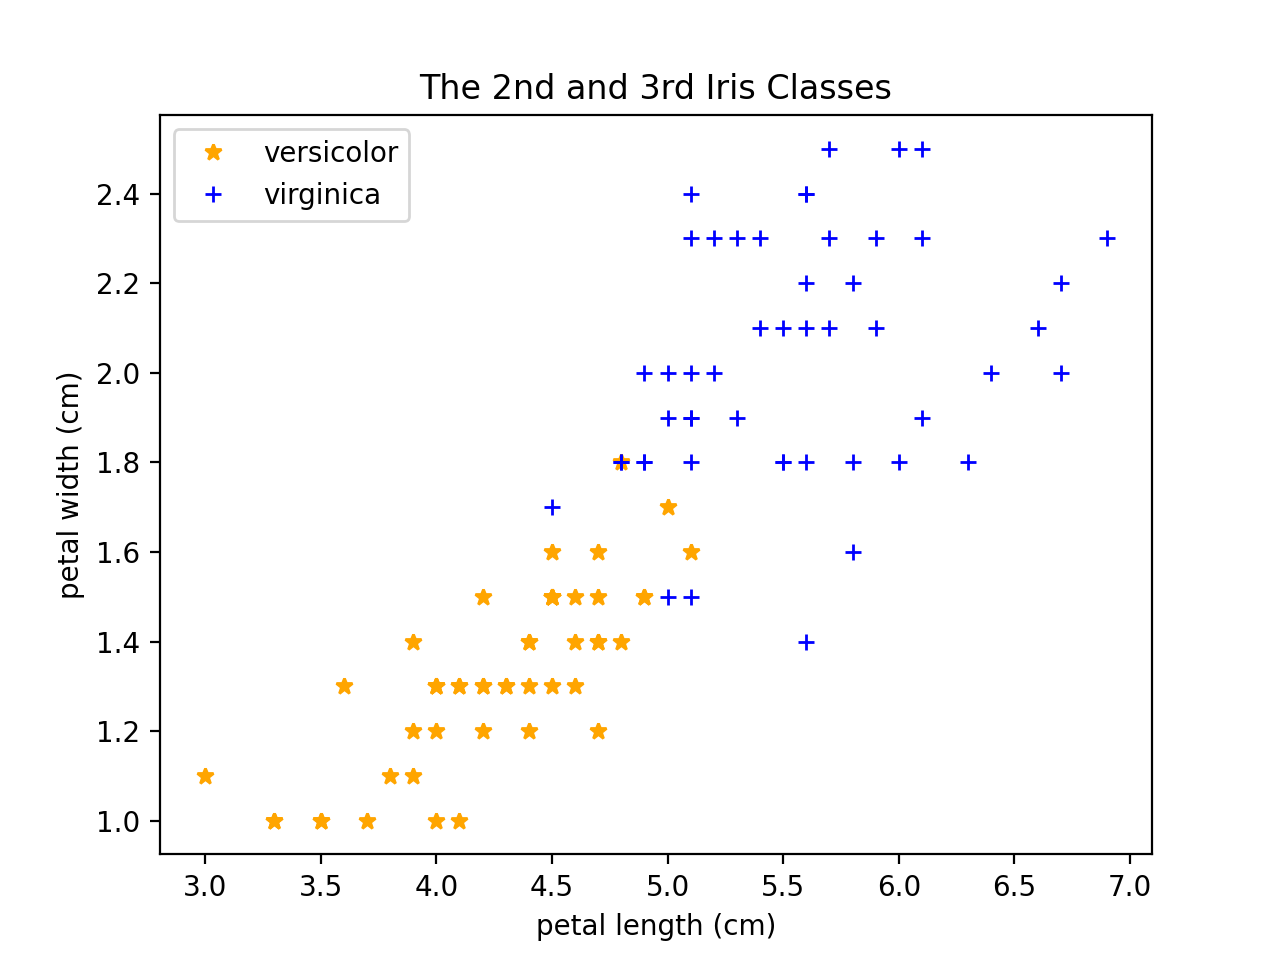
\includegraphics[scale=0.80]{ai1a}

The plot of 2nd and 3rd classes of the dataset with sepal width vs. sepal length:

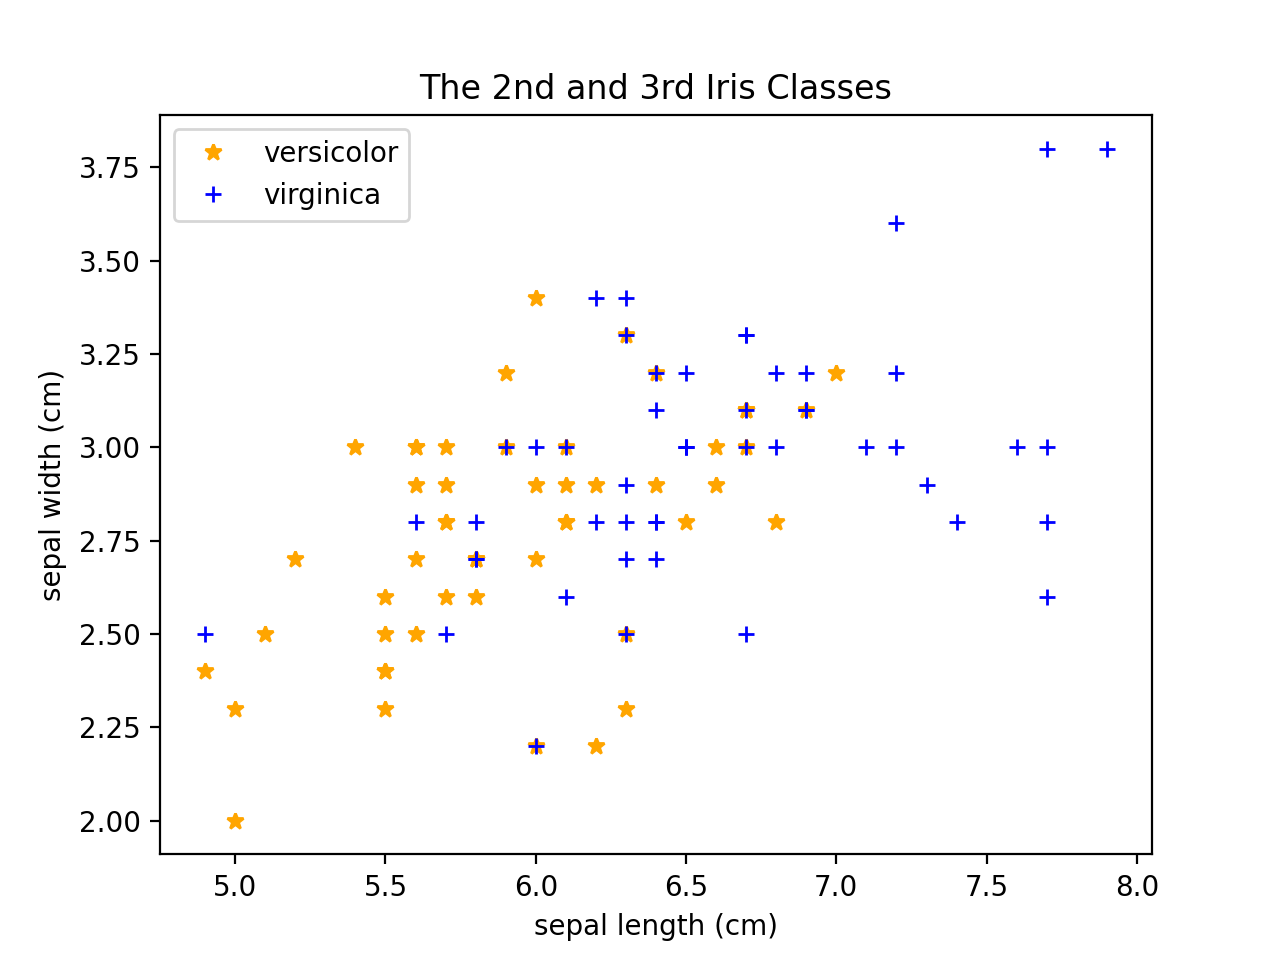
\includegraphics[scale=0.80]{ai1a2}

We can see that petal width vs. petal length can better seperate the 2nd and 3rd classes.

\subsection*{(b)}

We define the output unit: y = $w_1 \cdot$ petal\_length + $w_2 \cdot$ petal\_width + $w_0$

$w_1$ and $w_2$ are weigths, $w_0$ is bias.

The sigmoid function is $sigmoid = \dfrac{1}{1 + e^{-y}}$\\

sigmoind function code:\\

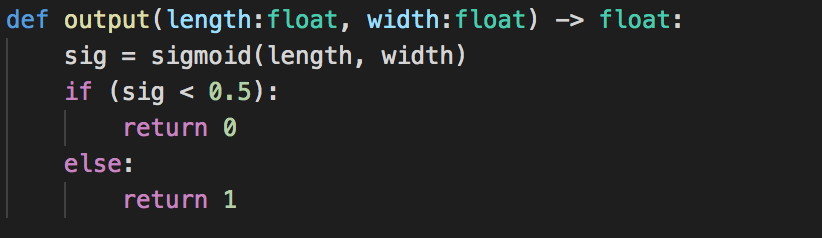
\includegraphics[scale=0.80]{ai1b2}

\subsection*{(c)}

Because the output unit is y = $w_1 \cdot$ petal\_length + $w_2 \cdot$ petal\_width + $w_0$ and the decision boundary is when y = 0, 

we use $x_1$ to represent petal length and $x_2$ to represent petal width: 

0 = $w_1 \cdot x_1 + w_2 \cdot x_2 + w_0$ \\

$x_2 = -\dfrac{w_1 \cdot x_1 + w_0}{w_2}$\\

decision boundary code:\\

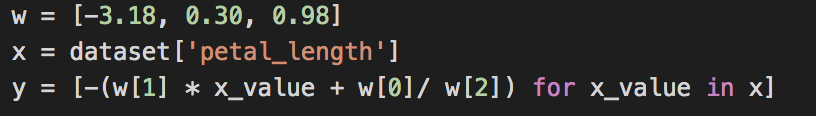
\includegraphics[scale=0.80]{ai1c2}

We draw the decision boundary on the graph using python: $plt.plot(x_1, x_2)$

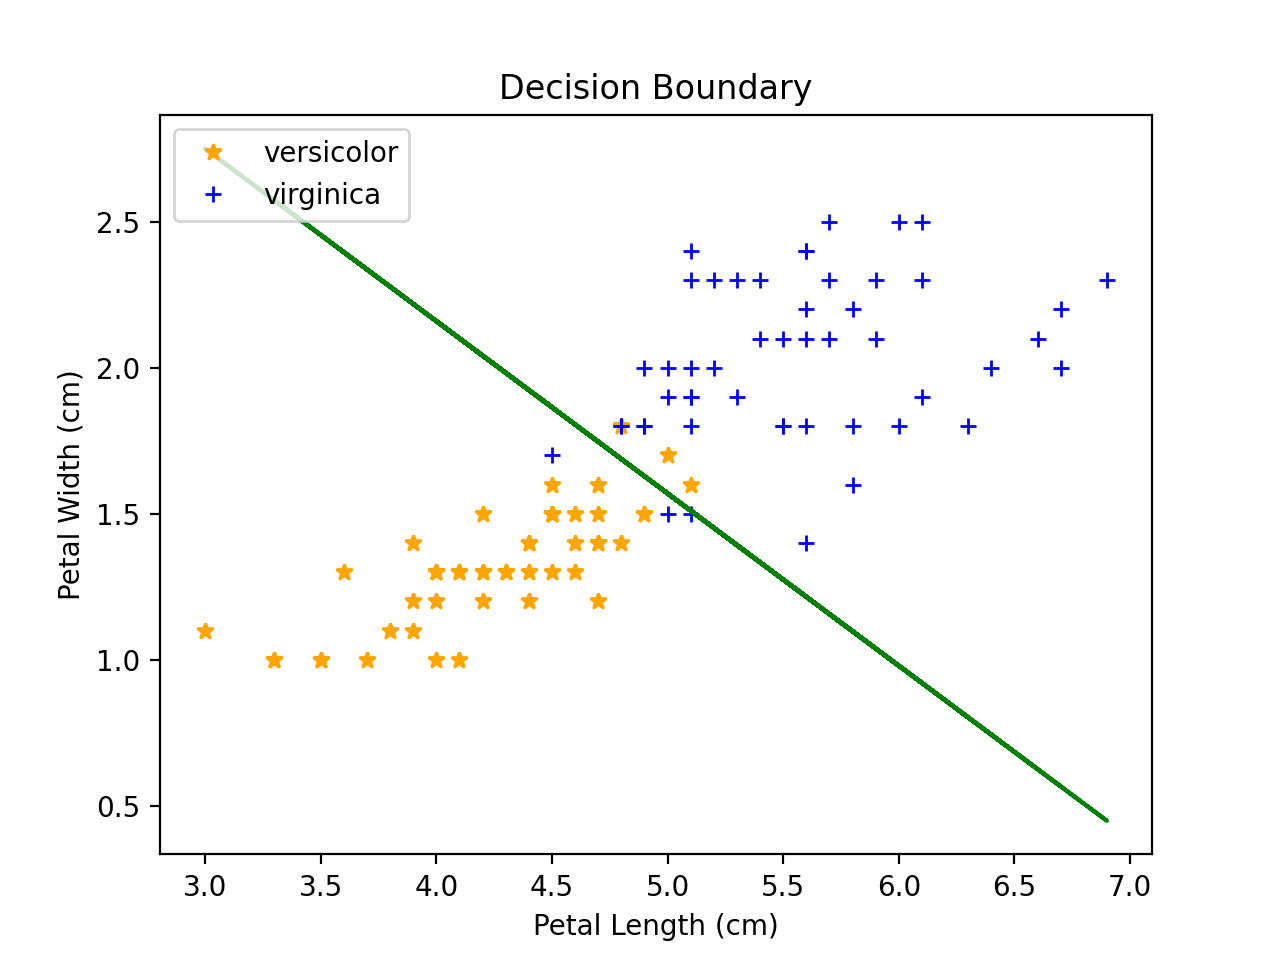
\includegraphics[scale=0.80]{ai1c}

\subsection*{(d)}

From the graph generated in (a), we can see that the range of petal length is from about 3.0 to 7.0 cm and the range of petal width is from about 1.0 to 2.5 cm,
so we set the range of petal length from 3.0 to 7.0 cm and the range of petal width from 1.0 to 2.5 cm for the surface that we are going to draw.

Then we use the output function we defined in (b) to calculate the output of each pair of petal length and petal width.

Code to prepare petal length, petal wieth, and the output:

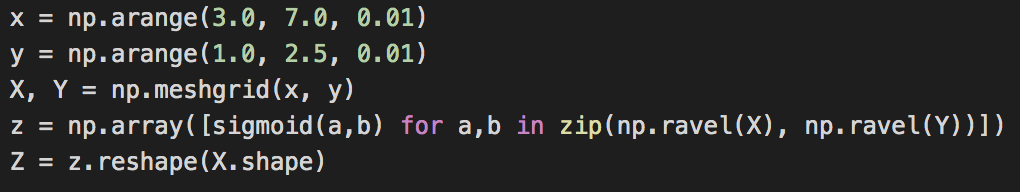
\includegraphics[scale=0.80]{ai1d2}

We use the petal length, petal wieth, and the output to draw a 3D neural network

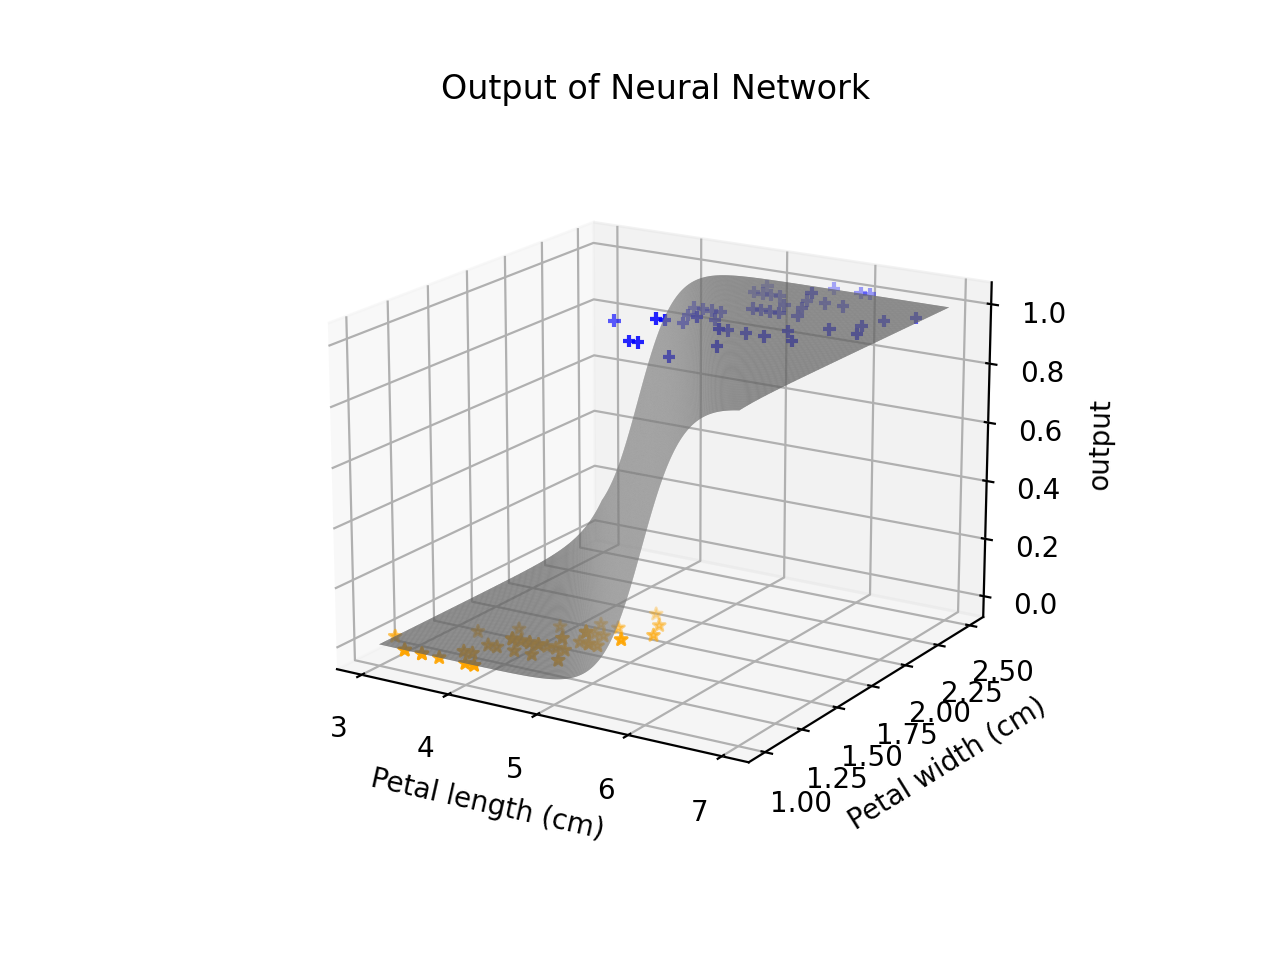
\includegraphics[scale=0.80]{ai1d}

\subsection*{(e)}

We selected 8 examples. 

\begin{tabular}{|l l l|}
    \hline
    petal length (cm) & petal width (cm) & species\\
    \hline
    4.8 & 1.8 & versicolor\\
    5.0 & 1.7 & versicolor\\
    3.5 & 1.0 & versicolor\\
    3.8 & 1.1 & versicolor\\
    5.1 & 1.8 & virginica \\
    5.0 & 1.5 & virginica \\
    4.9 & 1.8 & virginica \\
    5.9 & 2.3 & virginica \\
    \hline
\end{tabular}

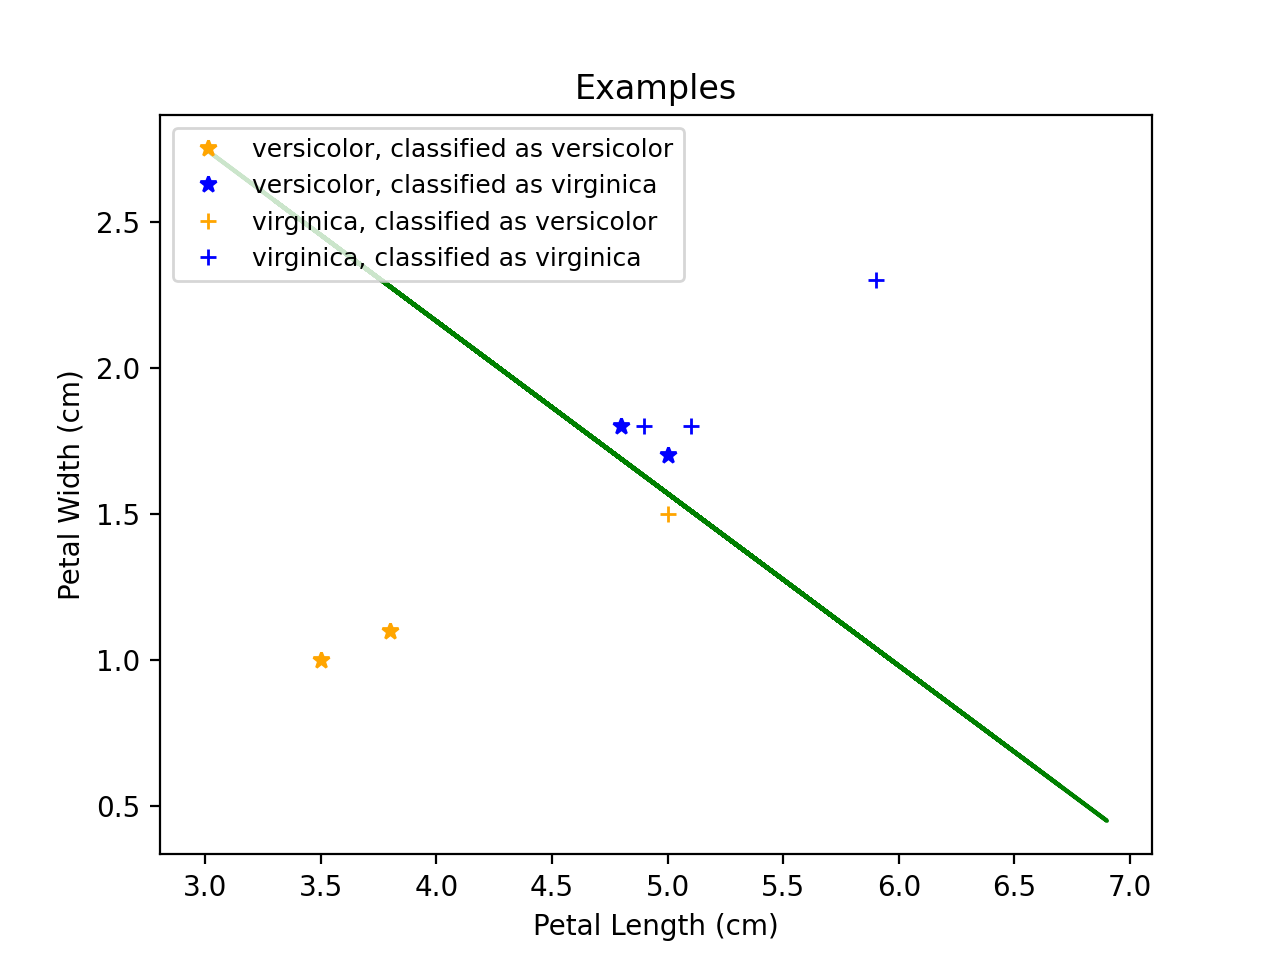
\includegraphics[scale=0.80]{ai1e}

\end{document}